\documentclass{article}

\usepackage[solutions]{xrcise}

\begin{document}
\sheet[2021]{Ersttermin}
\begin{exercise}{Kruskal-Algorithmus}
  Betrachten Sie den Graphen in \ref{fig:kruskal2021}. Bestimmen Sie mit Hilfe des Algorithmus von Kruskal einen minimalen Spannbaum des Graphen und skizzieren diesen. Geben Sie zusätzlich die Reihenfolge an, in der die Kanten des Spannbaums gemäß Algorithmus hinzugefügt werden.
  \begin{figure}
  \centering
  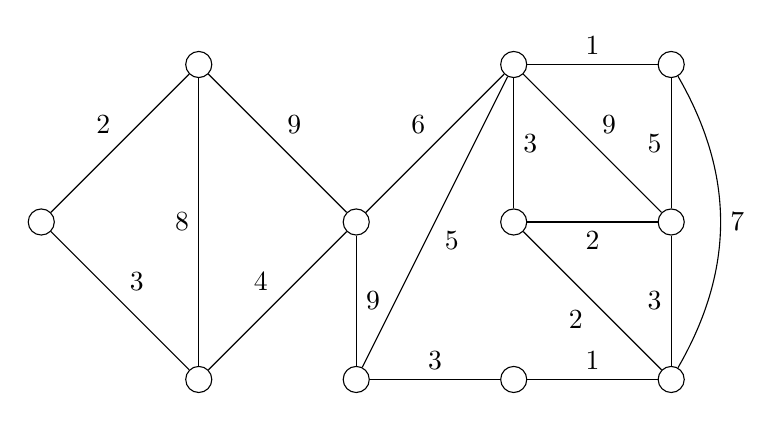
\begin{tikzpicture}[auto, node distance=2cm, main node/.style={circle, draw, minimum size=.5em}]
    \node[main node] (0) {};
    \node[main node] (1) [right of=0, below of=0] {};
    \node[main node] (2) [above of=1, above of=1] {};
    \node[main node] (3) [right of=2, below of=2] {};
    \node[main node] (4) [right of=3, above of=3] {};
    \node[main node] (5) [right of=4] {};
    \node[main node] (6) [below of=3] {};
    \node[main node] (7) [right of=6] {};
    \node[main node] (8) [right of=7] {};
    \node[main node] (9) [above of=8] {};
    \node[main node] (10) [left of=9] {};

    \path[every node]
    (0) edge node {3} (1)
    (0) edge node {2} (2)
    (1) edge node {8} (2)
    (1) edge node {4} (3)
    (2) edge node {9} (3)
    (3) edge node {6} (4)
    (3) edge node {9} (6)
    (4) edge node {1} (5)
    (4) edge node {5} (6)
    (4) edge node {9} (9)
    (4) edge node {3} (10)
    (5) edge[bend left] node {7} (8)
    (9) edge node {5} (5)
    (6) edge node {3} (7)
    (7) edge node {1} (8)
    (8) edge node {3} (9)
    (8) edge node {2} (10)
    (9) edge node {2} (10)
    ;
  \end{tikzpicture}

  \caption{Ein gewichteter Graph}\label{fig:kruskal}
\end{figure}

  \begin{solution}

  \end{solution}
\end{exercise}

\begin{exercise}{AVL-Bäume}
  Gegeben sei ein AVL-Baum für die Schlüssel $\{2,3,5,7,11,13,17,19\}$. Der Zustand der Datenstruktur ist in \ref{fig:avl} dargestellt. Skizzieren Sie die Datenstruktur nach dem Einfügen eines Elements mit Schlüssel 6 gemäß der Einfügeoperation aus der Vorlesung. Machen Sie dabei den jeweiligen Zustand vor und nach eventuell notwendigen Balancierungsschritten deutlich.
  \begin{figure}
  \centering
  \begin{tikzpicture}[auto,on grid,node distance=2cm,main node/.style={circle,draw,minimum size=0.75cm}]
    \node[main node] (5) {5};
    \node[main node, below left=of 5] (3) {3};
    \node[main node, below left=of 3] (2) {2};
    \node[main node, below right=of 5] (17) {17};
    \node[main node, below left=of 17] (11) {11};
    \node[main node, below right=of 17] (19) {19};
    \node[main node, below left=of 11] (7) {7};
    \node[main node, below right=of 11] (13) {13};

    \draw (5) -- (3) -- (2);
    \draw (5) -- (17) -- (11) -- (7);
    \draw (17) -- (19);
    \draw (11) -- (13);
  \end{tikzpicture}

  \caption{AVL-Baum für die Schlüssel $2, 3, 5, 7, 11, 13, 17, 19$.}\label{fig:avl}
\end{figure}

  \begin{solution}

  \end{solution}
\end{exercise}

\begin{exercise}{Big-O Notation}
  Jede der folgenden Teilaufgaben spezifiziert zwei Funktionen $f(n)$ und $g(n)$. Bestimmen Sie jeweils, ob die vier Relationen $f(n) = o(g(n))$, $f(n) = O(g(n))$, $f(n) = \Omega(g(n))$ und $f(n) = \omega(g(n))$ gelten (es sind also pro Teilaufgabe vier Antworten zu geben). Beweisen Sie Ihre Antwort jeweils kurz. Nutzen Sie dazu die Eigenschaften der asymptotischen Landau-Notation aus der Vorlesung (wie z. B. die Charakterisierung über Grenzwerte).
  \begin{enumerate}
    \item $f(n) = n \cdot (\log n)^{42}$ und $g(n) = n^{1.23}$
    \item $f(n) = n \cdot |\sin n|$ und $g(n) = \sqrt{n}$
    \item $f(n) = n^2 + n^{3/2} + n \cdot \log n$ und $g(n) = \binom{n}{2}$
    \item $f(n) = 8 \log n$ und $g(n) = n^3 \cdot \log n$
  \end{enumerate}
  \hint{Der Ausdruck $\binom{n}{k}$ bezeichnet den Binomialkoeffizienten $n$ über $k$. Die Basis des Logarithmus in Ausdrücken der Form $\log n$ ist 2.}

  \begin{solution}

  \end{solution}
\end{exercise}

\begin{exercise}{Union-Find Datenstruktur}
  Wir betrachten die Datenstruktur für disjunkte dynamische Mengen wie in der Vorlesung definiert. Die Grundmenge (das Universum) sei $U = \{a, b, . . . , z\}$, also die Menge der 26 Kleinbuchstaben $a$ bis $z$.
  \begin{enumerate}
    \item Geben Sie eine Folge von Aufrufen der Operationen MakeSet und Union an, welche die disjunkten Mengen $S_1 = \{a\}$, $S_2 = \{b, c, d\}$ sowie $S_3 = \{e, f\}$ erzeugt.
    \item Skizzieren Sie die Mengenobjekte der Datenstruktur, nachdem die disjunkten Mengen gemäß Ihrer Lösung zu Punkt (a) erzeugt wurden. Eine mögliche Darstellung ist in \ref{fig:unionFind} zu sehen.
    \item Geben Sie jeweils den Rückgabewert des Aufrufes FindSet(a) und des Aufrufes FindSet(d) an, nachdem die disjunkten Mengen gemäß Ihrer Lösung zu Punkt (a) erzeugt wurden.
    \item Skizzieren Sie das Mengenobjekt, welches entsteht, wenn nach Ihrer Lösung zu Punkt (a) die Operation Union(c,f) ausgeführt wird. Nutzen Sie wieder eine Darstellung ähnlich zu \ref{fig:unionFind}.
  \end{enumerate}
  \begin{figure}
  \centering
  \includegraphics[width=0.5\textwidth]{res/unionFind}

  \caption{Union-Find Datenstruktur}\label{fig:unionFind}
\end{figure}

  \begin{solution}

  \end{solution}
\end{exercise}

\begin{exercise}{Divide \& Conquer}
  Betrachten Sie den Divide \& Conquer Algorithmus, dessen Pseudocode in \ref{alg:Algo} gegeben ist und lösen Sie folgende Aufgaben:
  \begin{enumerate}
    \item Geben Sie eine Rekursionsgleichung für die Laufzeit $T(n)$ des Algorithmus bei Eingabe $(A, 1, n)$ für ein Array $A$ der Länge $n \in \mathbb{N}$ an.
    \item Analysieren Sie die Laufzeit von Algorithmus 1 möglichst genau in der $O$-Notation mit Hilfe der Substitutionsmethode. Sie können dabei annehmen, dass $n$ eine Zweierpotenz ist.
  \end{enumerate}
  \hint{Ein Induktionsbeweis der Laufzeit ist nicht notwendig, aber aus Ihrer Rechnung muss klar hervorgehen, wie Sie zu Ihrer Lösung kommen.}
  \begin{alg}
  % Algo(A, l, r)
  % n←r−l+1 ifn≤2
  % ifn=2
  % return |A[r] − A[l]|
  % else return 0 else
  % p←⌊(l+r)/2⌋
  % a ← Algo(A, l, p) b←Algo(A,p+1,r) ifa>b
  % c←a else c←b
  % fori←ltop
  % for j ← p + 1 to r
  % Lösung
  % (a)
  % Algorithmus 1
  % (Θ(1)
  % 2T (n/2) + Θ(n2)
  % return c
  % x ← |A[i] − A[j]| if x > c
  % c←x

\end{alg}

  \begin{solution}

  \end{solution}
\end{exercise}

\begin{exercise}{Datenstrukturen}
  Gesucht ist eine Datenstruktur, welche die drei folgenden Operationen unterstützt:
  \begin{itemize}
    \item \texttt{Einfügen}(x): Fügt die Zahl x in die Datenstruktur ein. Sie können zur Vereinfachung davon ausgehen, dass kein Element jemals doppelt in die Datenstruktur eingefügt wird.
    \item \texttt{Löschen}(x): Entfernt x, falls sich x in der Datenstruktur befindet. Andernfalls bleibt die Datenstruktur unverändert.
    \item \texttt{Rang}(x): Gibt die Anzahl der Elemente der Datenstruktur zurück, welche kleiner oder gleich x sind. Befinden sich z. B. die Zahlen $\{2,3,5,7,11,13\}$ in der Datenstruktur, so soll $Rang(5) = 3$ und $Rang(17) = 6$ gelten.
  \end{itemize}
  Die Datenstruktur soll alle drei Operationen in Laufzeit $O(\log n)$ unterstützen. Dabei bezeichnet $n$ die Anzahl der Elemente, die sich aktuell in der Datenstruktur befinden.\par
  Beschreiben Sie in wenigen kurzen Sätzen, wie Ihre Datenstruktur aufgebaut ist und wie die angegebenen Operationen realisiert werden. Hierbei ist kein Pseudocode gefordert. Es soll jedoch klar werden, dass die Datenstruktur korrekt arbeitet und die geforderte Laufzeit eingehalten wird.

  \begin{solution}

  \end{solution}
\end{exercise}

\begin{exercise}{Greedy-Algorithmen}
  Das Tankstopp-Problem modelliert die folgende Situation: Auf der Autofahrt von Ihrem Startpunkt $t_0$ bis zu Ihrem Ziel $t_n$ wollen Sie so wenige Tankstopps wie möglich einlegen. Unterwegs kommen Sie der Reihe nach an den Tankstellen $t_1,t_2,...,t_{n-1}$ vorbei. Sie starten mit vollem Tank und eine Tankfüllung Ihres Wagens reicht für $D$ Kilometer. Der Abstand zwischen den Tankstellen $t_{i-1}$ und $t_i$ beträgt $d_i$ Kilometer, wobei $0 < d_i \leq D$ gilt. Betrachten Sie die folgende Greedy-Strategie:
  \begin{quote}
    Fahre stets so weit wie möglich ohne Tankstopp und tanke erst an der am weitesten entfernten noch erreichbaren Tankstelle voll.
  \end{quote}
  Beweisen Sie, dass diese Greedy-Strategie eine optimale Lösung liefert, die Anzahl der Tankstopps also minimal ist.
  \hint{Die Lösung einer Strategie $A$, die $k$ Tankstopps benötigt, kann zum Beispiel als Folge von Indizes $a(1) < a(2) < \dots < a(k)$ mit $a(i) \in \{1,2,...,n\}$ beschrieben werden. Der $i$-te Tankstopp findet dabei an der Tankstelle $t_{a(i)}$ statt.}

  \begin{solution}

  \end{solution}
\end{exercise}

\begin{exercise}{NP-Vollständigkeit}
  Im Folgenden definieren wir zwei Entscheidungsprobleme:
  \begin{itemize}
    \item \textproblem{Unabhängige Menge}: Eine unabhängige Menge eines ungerichteten Graphen $G = (V,E)$ ist eine Teilmenge von Knoten $U \subseteq V$, so dass keine zwei Knoten aus $U$ adjazent sind. Es gilt also $\{u,v\} \in E$ für alle $u,v \in U$ mit $u \neq v$. Im Entscheidungsproblem \textproblem{Unabhängige Menge} ist ein kodiertes Paar $\langle G, k \rangle$ gegeben, wobei $G = (V,E)$ ein ungerichteter Graph ist und $k \in \mathbb{N}$. Es muss entschieden werden, ob $G$ eine unabhängige Menge $U \subseteq V$ der Größe $|U| \geq k$ enthält. Abbildung 4a zeigt ein Beispiel für eine Instanz des Problems.
    \item \textproblem{Keine Schnitte}: Gegeben ist ein kodiertes Paar $\langle S, l \rangle$, wobei $S = \{I_1, I_2, \dots\}$ eine endliche Menge von Intervallen $I_i \subseteq \mathbb{R}$ ist und $l \in \mathbb{N}$. Es muss entschieden werden, ob es eine Teilmenge $T \subseteq S$ von $S$ der Größe $|T| \geq l$ gibt, so dass alle Intervalle in $T$ paarweise disjunkt sind.
  \end{itemize}
  \hint{Sie dürfen zur Lösung der folgenden Aufgaben benutzen, dass \textproblem{Unabhängige Menge} NP-schwer ist.}
  \begin{enumerate}
    \item Ist \textproblem{Unabhängige Menge} NP-vollständig? Beweisen Sie Ihre Antwort.
    \item Beweisen Sie \textproblem{Keine Schnitte} $\leq_P$ \textproblem{Unabhängige Menge}.
    \item Was folgt daraus für die Komplexität von \textproblem{Keine Schnitte}?
  \end{enumerate}

  \begin{solution}

  \end{solution}
\end{exercise}
\end{document}